% %%%%%%%%%%%%%%%%%%%%%%%%%%%%%%%%%%%%%%%%%%%%%%%%%%%%%%%%%%%%%%%%%%%%%%%%%%%%%%%%%%%%%%%%%%%%
% PROBLEM SET LATEX TEMPLATE FILE
% DEFINE DOCUMENT STYLE, LOAD PACKAGES
\documentclass[11pt,notitlepage]{article}\usepackage[]{graphicx}\usepackage[]{color}
%% maxwidth is the original width if it is less than linewidth
%% otherwise use linewidth (to make sure the graphics do not exceed the margin)
\makeatletter
\def\maxwidth{ %
  \ifdim\Gin@nat@width>\linewidth
    \linewidth
  \else
    \Gin@nat@width
  \fi
}
\makeatother

\definecolor{fgcolor}{rgb}{0.345, 0.345, 0.345}
\newcommand{\hlnum}[1]{\textcolor[rgb]{0.686,0.059,0.569}{#1}}%
\newcommand{\hlstr}[1]{\textcolor[rgb]{0.192,0.494,0.8}{#1}}%
\newcommand{\hlcom}[1]{\textcolor[rgb]{0.678,0.584,0.686}{\textit{#1}}}%
\newcommand{\hlopt}[1]{\textcolor[rgb]{0,0,0}{#1}}%
\newcommand{\hlstd}[1]{\textcolor[rgb]{0.345,0.345,0.345}{#1}}%
\newcommand{\hlkwa}[1]{\textcolor[rgb]{0.161,0.373,0.58}{\textbf{#1}}}%
\newcommand{\hlkwb}[1]{\textcolor[rgb]{0.69,0.353,0.396}{#1}}%
\newcommand{\hlkwc}[1]{\textcolor[rgb]{0.333,0.667,0.333}{#1}}%
\newcommand{\hlkwd}[1]{\textcolor[rgb]{0.737,0.353,0.396}{\textbf{#1}}}%

\usepackage{framed}
\makeatletter
\newenvironment{kframe}{%
 \def\at@end@of@kframe{}%
 \ifinner\ifhmode%
  \def\at@end@of@kframe{\end{minipage}}%
  \begin{minipage}{\columnwidth}%
 \fi\fi%
 \def\FrameCommand##1{\hskip\@totalleftmargin \hskip-\fboxsep
 \colorbox{shadecolor}{##1}\hskip-\fboxsep
     % There is no \\@totalrightmargin, so:
     \hskip-\linewidth \hskip-\@totalleftmargin \hskip\columnwidth}%
 \MakeFramed {\advance\hsize-\width
   \@totalleftmargin\z@ \linewidth\hsize
   \@setminipage}}%
 {\par\unskip\endMakeFramed%
 \at@end@of@kframe}
\makeatother

\definecolor{shadecolor}{rgb}{.97, .97, .97}
\definecolor{messagecolor}{rgb}{0, 0, 0}
\definecolor{warningcolor}{rgb}{1, 0, 1}
\definecolor{errorcolor}{rgb}{1, 0, 0}
\newenvironment{knitrout}{}{} % an empty environment to be redefined in TeX

\usepackage{alltt}    % ADD COMMENTS USING A PERCENT SIGN
\usepackage{amsfonts}
\usepackage{amsthm}
\usepackage{amsmath, booktabs}
\usepackage{mathtools}
\usepackage{amssymb}
\usepackage{subfig}
\usepackage{setspace}
\usepackage{fullpage}
\usepackage{verbatim}
\usepackage{graphicx}
\usepackage{tabularx}
\usepackage{longtable}
\usepackage{multicol}
\usepackage{multirow}
\setlength{\parindent}{0in}  	% uncomment to remove indent at start of paragraphs
\usepackage{pdflscape}
\usepackage[english]{babel}
\usepackage[pdftex]{hyperref}
\usepackage{natbib}
\usepackage{caption}
\usepackage{amsmath}
\usepackage{amsfonts}
\usepackage{graphics}
\usepackage{multirow}
\usepackage{graphics}
\usepackage{hyperref}
\usepackage{longtable}
\usepackage{latexsym}
\usepackage{rotating}
\usepackage{setspace}
\usepackage{layouts} 
\usepackage[titletoc]{appendix}
\DeclareGraphicsExtensions{.pdf,.jpg,.png}
\usepackage[margin=1in]{geometry}
\usepackage{enumerate}
\usepackage{float}

\newcolumntype{L}[1]{>{\raggedright\let\newline\\\arraybackslash\hspace{0pt}}m{#1}}
\newcolumntype{C}[1]{>{\centering\let\newline\\\arraybackslash\hspace{0pt}}m{#1}}
\newcolumntype{R}[1]{>{\raggedleft\let\newline\\\arraybackslash\hspace{0pt}}m{#1}}

\usepackage[T1]{fontenc}

\usepackage{xcolor}
\usepackage[printwatermark]{xwatermark}

\usepackage{textcomp} % defines textquotesingle
 \AtBeginDocument{%
        \def\PYZsq{\textquotesingle}% Upright quotes in Pygmentized code
    }
 
 \usepackage{fancyvrb} % verbatim replacement that allows latex
    % Hack from http://tex.stackexchange.com/a/47451/13684:
    \AtBeginDocument{%
        \def\PYZsq{\textquotesingle}% Upright quotes in Pygmentized code
    }
    \usepackage{upquote} % Upright quotes for verbatim code
 


    % Pygments definitions
    
\makeatletter
\def\PY@reset{\let\PY@it=\relax \let\PY@bf=\relax%
    \let\PY@ul=\relax \let\PY@tc=\relax%
    \let\PY@bc=\relax \let\PY@ff=\relax}
\def\PY@tok#1{\csname PY@tok@#1\endcsname}
\def\PY@toks#1+{\ifx\relax#1\empty\else%
    \PY@tok{#1}\expandafter\PY@toks\fi}
\def\PY@do#1{\PY@bc{\PY@tc{\PY@ul{%
    \PY@it{\PY@bf{\PY@ff{#1}}}}}}}
\def\PY#1#2{\PY@reset\PY@toks#1+\relax+\PY@do{#2}}

\expandafter\def\csname PY@tok@w\endcsname{\def\PY@tc##1{\textcolor[rgb]{0.73,0.73,0.73}{##1}}}
\expandafter\def\csname PY@tok@c\endcsname{\let\PY@it=\textit\def\PY@tc##1{\textcolor[rgb]{0.25,0.50,0.50}{##1}}}
\expandafter\def\csname PY@tok@cp\endcsname{\def\PY@tc##1{\textcolor[rgb]{0.74,0.48,0.00}{##1}}}
\expandafter\def\csname PY@tok@k\endcsname{\let\PY@bf=\textbf\def\PY@tc##1{\textcolor[rgb]{0.00,0.50,0.00}{##1}}}
\expandafter\def\csname PY@tok@kp\endcsname{\def\PY@tc##1{\textcolor[rgb]{0.00,0.50,0.00}{##1}}}
\expandafter\def\csname PY@tok@kt\endcsname{\def\PY@tc##1{\textcolor[rgb]{0.69,0.00,0.25}{##1}}}
\expandafter\def\csname PY@tok@o\endcsname{\def\PY@tc##1{\textcolor[rgb]{0.40,0.40,0.40}{##1}}}
\expandafter\def\csname PY@tok@ow\endcsname{\let\PY@bf=\textbf\def\PY@tc##1{\textcolor[rgb]{0.67,0.13,1.00}{##1}}}
\expandafter\def\csname PY@tok@nb\endcsname{\def\PY@tc##1{\textcolor[rgb]{0.00,0.50,0.00}{##1}}}
\expandafter\def\csname PY@tok@nf\endcsname{\def\PY@tc##1{\textcolor[rgb]{0.00,0.00,1.00}{##1}}}
\expandafter\def\csname PY@tok@nc\endcsname{\let\PY@bf=\textbf\def\PY@tc##1{\textcolor[rgb]{0.00,0.00,1.00}{##1}}}
\expandafter\def\csname PY@tok@nn\endcsname{\let\PY@bf=\textbf\def\PY@tc##1{\textcolor[rgb]{0.00,0.00,1.00}{##1}}}
\expandafter\def\csname PY@tok@ne\endcsname{\let\PY@bf=\textbf\def\PY@tc##1{\textcolor[rgb]{0.82,0.25,0.23}{##1}}}
\expandafter\def\csname PY@tok@nv\endcsname{\def\PY@tc##1{\textcolor[rgb]{0.10,0.09,0.49}{##1}}}
\expandafter\def\csname PY@tok@no\endcsname{\def\PY@tc##1{\textcolor[rgb]{0.53,0.00,0.00}{##1}}}
\expandafter\def\csname PY@tok@nl\endcsname{\def\PY@tc##1{\textcolor[rgb]{0.63,0.63,0.00}{##1}}}
\expandafter\def\csname PY@tok@ni\endcsname{\let\PY@bf=\textbf\def\PY@tc##1{\textcolor[rgb]{0.60,0.60,0.60}{##1}}}
\expandafter\def\csname PY@tok@na\endcsname{\def\PY@tc##1{\textcolor[rgb]{0.49,0.56,0.16}{##1}}}
\expandafter\def\csname PY@tok@nt\endcsname{\let\PY@bf=\textbf\def\PY@tc##1{\textcolor[rgb]{0.00,0.50,0.00}{##1}}}
\expandafter\def\csname PY@tok@nd\endcsname{\def\PY@tc##1{\textcolor[rgb]{0.67,0.13,1.00}{##1}}}
\expandafter\def\csname PY@tok@s\endcsname{\def\PY@tc##1{\textcolor[rgb]{0.73,0.13,0.13}{##1}}}
\expandafter\def\csname PY@tok@sd\endcsname{\let\PY@it=\textit\def\PY@tc##1{\textcolor[rgb]{0.73,0.13,0.13}{##1}}}
\expandafter\def\csname PY@tok@si\endcsname{\let\PY@bf=\textbf\def\PY@tc##1{\textcolor[rgb]{0.73,0.40,0.53}{##1}}}
\expandafter\def\csname PY@tok@se\endcsname{\let\PY@bf=\textbf\def\PY@tc##1{\textcolor[rgb]{0.73,0.40,0.13}{##1}}}
\expandafter\def\csname PY@tok@sr\endcsname{\def\PY@tc##1{\textcolor[rgb]{0.73,0.40,0.53}{##1}}}
\expandafter\def\csname PY@tok@ss\endcsname{\def\PY@tc##1{\textcolor[rgb]{0.10,0.09,0.49}{##1}}}
\expandafter\def\csname PY@tok@sx\endcsname{\def\PY@tc##1{\textcolor[rgb]{0.00,0.50,0.00}{##1}}}
\expandafter\def\csname PY@tok@m\endcsname{\def\PY@tc##1{\textcolor[rgb]{0.40,0.40,0.40}{##1}}}
\expandafter\def\csname PY@tok@gh\endcsname{\let\PY@bf=\textbf\def\PY@tc##1{\textcolor[rgb]{0.00,0.00,0.50}{##1}}}
\expandafter\def\csname PY@tok@gu\endcsname{\let\PY@bf=\textbf\def\PY@tc##1{\textcolor[rgb]{0.50,0.00,0.50}{##1}}}
\expandafter\def\csname PY@tok@gd\endcsname{\def\PY@tc##1{\textcolor[rgb]{0.63,0.00,0.00}{##1}}}
\expandafter\def\csname PY@tok@gi\endcsname{\def\PY@tc##1{\textcolor[rgb]{0.00,0.63,0.00}{##1}}}
\expandafter\def\csname PY@tok@gr\endcsname{\def\PY@tc##1{\textcolor[rgb]{1.00,0.00,0.00}{##1}}}
\expandafter\def\csname PY@tok@ge\endcsname{\let\PY@it=\textit}
\expandafter\def\csname PY@tok@gs\endcsname{\let\PY@bf=\textbf}
\expandafter\def\csname PY@tok@gp\endcsname{\let\PY@bf=\textbf\def\PY@tc##1{\textcolor[rgb]{0.00,0.00,0.50}{##1}}}
\expandafter\def\csname PY@tok@go\endcsname{\def\PY@tc##1{\textcolor[rgb]{0.53,0.53,0.53}{##1}}}
\expandafter\def\csname PY@tok@gt\endcsname{\def\PY@tc##1{\textcolor[rgb]{0.00,0.27,0.87}{##1}}}
\expandafter\def\csname PY@tok@err\endcsname{\def\PY@bc##1{\setlength{\fboxsep}{0pt}\fcolorbox[rgb]{1.00,0.00,0.00}{1,1,1}{\strut ##1}}}
\expandafter\def\csname PY@tok@kc\endcsname{\let\PY@bf=\textbf\def\PY@tc##1{\textcolor[rgb]{0.00,0.50,0.00}{##1}}}
\expandafter\def\csname PY@tok@kd\endcsname{\let\PY@bf=\textbf\def\PY@tc##1{\textcolor[rgb]{0.00,0.50,0.00}{##1}}}
\expandafter\def\csname PY@tok@kn\endcsname{\let\PY@bf=\textbf\def\PY@tc##1{\textcolor[rgb]{0.00,0.50,0.00}{##1}}}
\expandafter\def\csname PY@tok@kr\endcsname{\let\PY@bf=\textbf\def\PY@tc##1{\textcolor[rgb]{0.00,0.50,0.00}{##1}}}
\expandafter\def\csname PY@tok@bp\endcsname{\def\PY@tc##1{\textcolor[rgb]{0.00,0.50,0.00}{##1}}}
\expandafter\def\csname PY@tok@fm\endcsname{\def\PY@tc##1{\textcolor[rgb]{0.00,0.00,1.00}{##1}}}
\expandafter\def\csname PY@tok@vc\endcsname{\def\PY@tc##1{\textcolor[rgb]{0.10,0.09,0.49}{##1}}}
\expandafter\def\csname PY@tok@vg\endcsname{\def\PY@tc##1{\textcolor[rgb]{0.10,0.09,0.49}{##1}}}
\expandafter\def\csname PY@tok@vi\endcsname{\def\PY@tc##1{\textcolor[rgb]{0.10,0.09,0.49}{##1}}}
\expandafter\def\csname PY@tok@vm\endcsname{\def\PY@tc##1{\textcolor[rgb]{0.10,0.09,0.49}{##1}}}
\expandafter\def\csname PY@tok@sa\endcsname{\def\PY@tc##1{\textcolor[rgb]{0.73,0.13,0.13}{##1}}}
\expandafter\def\csname PY@tok@sb\endcsname{\def\PY@tc##1{\textcolor[rgb]{0.73,0.13,0.13}{##1}}}
\expandafter\def\csname PY@tok@sc\endcsname{\def\PY@tc##1{\textcolor[rgb]{0.73,0.13,0.13}{##1}}}
\expandafter\def\csname PY@tok@dl\endcsname{\def\PY@tc##1{\textcolor[rgb]{0.73,0.13,0.13}{##1}}}
\expandafter\def\csname PY@tok@s2\endcsname{\def\PY@tc##1{\textcolor[rgb]{0.73,0.13,0.13}{##1}}}
\expandafter\def\csname PY@tok@sh\endcsname{\def\PY@tc##1{\textcolor[rgb]{0.73,0.13,0.13}{##1}}}
\expandafter\def\csname PY@tok@s1\endcsname{\def\PY@tc##1{\textcolor[rgb]{0.73,0.13,0.13}{##1}}}
\expandafter\def\csname PY@tok@mb\endcsname{\def\PY@tc##1{\textcolor[rgb]{0.40,0.40,0.40}{##1}}}
\expandafter\def\csname PY@tok@mf\endcsname{\def\PY@tc##1{\textcolor[rgb]{0.40,0.40,0.40}{##1}}}
\expandafter\def\csname PY@tok@mh\endcsname{\def\PY@tc##1{\textcolor[rgb]{0.40,0.40,0.40}{##1}}}
\expandafter\def\csname PY@tok@mi\endcsname{\def\PY@tc##1{\textcolor[rgb]{0.40,0.40,0.40}{##1}}}
\expandafter\def\csname PY@tok@il\endcsname{\def\PY@tc##1{\textcolor[rgb]{0.40,0.40,0.40}{##1}}}
\expandafter\def\csname PY@tok@mo\endcsname{\def\PY@tc##1{\textcolor[rgb]{0.40,0.40,0.40}{##1}}}
\expandafter\def\csname PY@tok@ch\endcsname{\let\PY@it=\textit\def\PY@tc##1{\textcolor[rgb]{0.25,0.50,0.50}{##1}}}
\expandafter\def\csname PY@tok@cm\endcsname{\let\PY@it=\textit\def\PY@tc##1{\textcolor[rgb]{0.25,0.50,0.50}{##1}}}
\expandafter\def\csname PY@tok@cpf\endcsname{\let\PY@it=\textit\def\PY@tc##1{\textcolor[rgb]{0.25,0.50,0.50}{##1}}}
\expandafter\def\csname PY@tok@c1\endcsname{\let\PY@it=\textit\def\PY@tc##1{\textcolor[rgb]{0.25,0.50,0.50}{##1}}}
\expandafter\def\csname PY@tok@cs\endcsname{\let\PY@it=\textit\def\PY@tc##1{\textcolor[rgb]{0.25,0.50,0.50}{##1}}}

\def\PYZbs{\char`\\}
\def\PYZus{\char`\_}
\def\PYZob{\char`\{}
\def\PYZcb{\char`\}}
\def\PYZca{\char`\^}
\def\PYZam{\char`\&}
\def\PYZlt{\char`\<}
\def\PYZgt{\char`\>}
\def\PYZsh{\char`\#}
\def\PYZpc{\char`\%}
\def\PYZdl{\char`\$}
\def\PYZhy{\char`\-}
\def\PYZsq{\char`\'}
\def\PYZdq{\char`\"}
\def\PYZti{\char`\~}
% for compatibility with earlier versions
\def\PYZat{@}
\def\PYZlb{[}
\def\PYZrb{]}
\makeatother


    % Exact colors from NB
    \definecolor{incolor}{rgb}{0.0, 0.0, 0.5}
    \definecolor{outcolor}{rgb}{0.545, 0.0, 0.0}
    
    \providecommand{\tightlist}{%
      \setlength{\itemsep}{0pt}\setlength{\parskip}{0pt}}
\DefineVerbatimEnvironment{Highlighting}{Verbatim}{commandchars=\\\{\}}



    




\title{Field Experiments: Design, Analysis and Interpretation \\
Solutions for Chapter 12 Exercises}
\author{Alan S. Gerber and Donald P. Green\footnote{Solutions prepared by Peter M. Aronow and revised by Alexander Coppock}}
\date{\vspace{-5ex}}

%%%%%%%%%%%%%%%%%%%%%%%%%%%%%%%%%%%%%%%%%%%%%%%%%%%%%%%%%%%%%%%%%%%%%%%%%%%%%%%%%%%%%%%%%%%%%
\IfFileExists{upquote.sty}{\usepackage{upquote}}{}
\begin{document}

\maketitle


\section*{Question 1}
Stewart Page performed an audit study to measure the extent to which gay people encounter discrimination in the rental housing market.\footnote{Page 1998.} Answer the following questions, which direct your attention to specific page numbers in the original article.

\begin{enumerate}[a)]
\item Who are the subjects in this experiment (p. 33)?\\
Answer:\\
The subjects are landlords who advertised rental housing in two Canadian cities (Windsor and London, Ontario; N=60 for each city) and Detroit Michigan (N=60). The landlords were selected based on advertisements they placed for rental property in the classified ads section of the most recently available newspaper in each city. It is not clear how the sample was drawn from the available ads, except that some restrictions are described: advertisements were excluded if there was no phone number listed in the ad or if the ad listed preferences or specific conditions for prospective tenants. In addition, once the experiment was underway subjects were discarded if they did not understand the meaning of the call (page 34). It is unclear, but it appears that subjects were dropped if the caller could not reach the landlord, either because the line was repeatedly busy or not answered. Finally, subjects were dropped if the person who was reached was either not in charge of renting the room or was authorized to give a definite answer regarding its availability (see p. 33). After these exclusions, there remained 180 landlords (assuming that no landlord in the sample was associated with more than one rental property). 

\item What is the treatment (pp. 33-34)?\\
Answer:\\
Subjects were assigned to receive the control call (an inquiry about the current availability of the advertised apartment) or the treatment call (an inquiry about the availability of the apartment prefaced by the statement: ``I guess it's only fair to tell you that I'm a gay person'' (or ``a lesbian''). For each city 30 calls were made by a male caller and 30 by a female caller (p. 33). Thus there was assignment into 4 groups (gender x sexual orientation) with 15 subjects in each group in each city. Both caller gender and the sexual orientation prompt may both be considered as treatments. According to the write up, there was no fixed script but calls were kept ``as brief as possible, generally of only seconds in duration, and were limited to direct inquiries.'' (p. 33).   

\item One criticism of audit studies is that in addition to differing with respect to the intended treatment (in this case, sexual orientation of the renter), the treatment and control group also differ in other ways that might be related to the outcome variable. What is the technical name for the assumption that audit studies may violate?\\
Answer:\\
Audit studies may violate the exclusion restriction. Let Y be the stated availability of the apartment, D the presumed sexual orientation of the potential renter, and Z the assignment to the treatment or control script. If the script intended to convey a gay sexual orientation (D) strikes the landlord as disagreeably defensive or odd in the context of a call regarding the rental property, for example, then Z may affect Y through pathways other than the putative sexual orientation of the prospective tenant. Similarly, if those making the calls have a viewpoint regarding anti-gay bias, this may affect how the calls are delivered apart from conveying the sexual orientation of the potential renter.

\item Suppose that the experiment used one male caller to make calls that mentioned sexual orientation and another male caller to make calls that did not. How would this procedure affect your interpretation of the apparent degree of discrimination against gay men?\\
Answer:\\
There would be a potential violation of the exclusion restriction. If there are two callers, the difference in average outcomes for the straight and gay script groups will estimate the effect of the combination of the qualities of person 1 and the gay orientation script versus the qualities of person 2 and no gay orientation prompt. Unless there is no difference in how renters respond to person 1 versus person 2, this estimand is not the average effect of sexual orientation. 

\item Take a careful look at the treatment and control scripts, and consider some ways that the treatment and control conditions might differ in addition to transmitting information about the potential renter's sexual orientation. Are the scripts the same length? Do both scripts seem similar in terms of tone and style? How might the incidental differences between scripts affect the generalizations that can be drawn from this study?\\
Answer:\\

Suppose the goal is to use the findings to draw conclusions about the gay person's real world experience when calling a landlord who is made aware of the caller's sexual orientation about the availability of an apartment. To evaluate generalizability, we consider whether the scripts parallel what a gay and straight person might actually say to a potential landlord and whether, in instances in which the scripts deviate from this, any deviations might affect potential outcomes.  

The gay and straight scripts are different in several ways in addition to conveying different sexual orientations. The script with the sexual orientation prompt contains more information than the control script and is also longer. It is unlikely that these difference parallel real world differences in how a gay versus straight person will interact with a landlord, and so if these differences matter for landlord response this will compromise the generalizability of the experiment. However, it is unlikely that these differences are important in this particular context. Raising the issue of sexual orientation in a preliminary inquiry may convey a degree of assertiveness, political commitment, or a lifestyle that might have an independent effect on the desirability of the potential tenant apart from the particular question of sexual orientation.  If sharing one's sexual orientation in a preliminary phone call is not a common feature in real rental experiences, and this script feature is considered odd or shocking by some landlords, the results may not generalize to the typical real world rental experience. 

\item How might you design an experiment to eliminate some or all of these incidental differences between scripts?\\
Answer:\\
A key design challenge in this experiment is conveying sexual orientation in a brief interaction in a naturalistic way. A treatment script that used an indirect strategy would not have the same potential to carry the baggage (convey assertiveness, etc.) that is incidental to the intended treatment. For instance, a script that referred to the potential renter's boyfriend or girlfriend (``the location is great because my boyfriend/girlfriend goes to school or works in the neighborhood'') might convey sexual orientation in a more subtle fashion. This script strategy also has the benefit of eliminating differences in script length and information content. 

Given that any particular script for conveying sexual orientation might be less than ideal, the researcher might diversify and try a variety of indirect methods and see if the effects are different across scripts. If the scripts are equally effective, this suggests that the common element across the scripts (sexual orientation) rather than idiosyncratic features of the scripts is driving any results you observe.  

\item Based on the description on pages 33-34, how are subjects assigned to the treatment groups? What is the implication if random assignment was not used?\\
Answer:\\
The allocation to groups is described as follows: ``Calls to the same city were assigned to the two conditions by way of systematic alternation of telephone numbers.'' It is not entirely clear what this entails. Suppose it means that the list for a city was first sorted in ascending order by phone number and then the subjects were assigned to each of the 4 conditions in an alternating fashion such that the first number (and fifth and ninth etc.) was assigned to, say, the no gay prompt and male caller group. 

If telephone numbers are randomly assigned to landlords and the order of assignment to the 4 treatment and control groups was independent of the telephone numbers, the alternation method is equivalent to random assignment. 

However, it is (theoretically) possible that the allocation method is not equivalent to random assignment. First, subject potential outcomes may be correlated with phone numbers.  If so, the sampling distribution produced by randomization inference under the sharp null will be incorrect. Second, if there is a relationship between the potential outcomes and telephone numbers, it is possible that conscious or unconscious bias might lead the researcher to assign some  numbers to certain groups, which will lead to biased estimates. 

\end{enumerate}

\section*{Question 2}
\begin{knitrout}
\definecolor{shadecolor}{rgb}{0.969, 0.969, 0.969}\color{fgcolor}\begin{kframe}
\begin{verbatim}






\end{verbatim}
\end{kframe}
\end{knitrout}


\section*{Question 3}
In an experiment designed to evaluate the effects of political institutions, Olken randomly assigned 49 villages in Indonesia to alternative political processes for selecting development projects.\footnote{Olken 2010.} Some villages were assigned to the status quo selection procedure (village meetings with low attendance), while others were assigned to use an innovative method of direct elections (a village-wide plebiscite). Consistent with expectations, participation in the plebiscite was 20 times greater than attendance at the village meetings. Olken examines the new procedure's effect on which projects are selected and how the villagers feel about the selection process. He finds that there are minimal changes in which projects are selected. However, a survey after the project selection found that the villagers who were assigned to the plebiscite reported much greater satisfaction with the project selection process, and were significantly more likely to view the selection as fair, and the project as useful and in accordance with their own and the people's wishes.

\begin{enumerate}[a)]

\item One part of this experiment focuses on whether the treatment influences which projects villages select. These results are reported in Figure 1, and the study is described on pp. 244-247. Describe the experimental subjects. What units are assigned to treatment versus control? What is the treatment?\\
Answer:\\

The subjects are 49 villages in Indonesia. Villages in three regions were randomly assigned to treatment or control: North Sumatra (5 plebiscite, 14 meeting), East Java (3 plebiscite, 7 meeting) and Southeast Sulawesi (9 plebiscite, 11 meeting). These villages are all eligible to propose development projects for possible funding through a government program. The treatment involves altering the process whereby villages select which projects they will propose for funding. The standard method (control group) involves assembling two lists of possible projects (a general project selected from the ideas produced by meetings attended by men or by both genders and a women's project selected from ideas produced by meetings of women). The final step in the project proposal process is to take the list of project ideas to sparsely attended general meetings (one to which the whole village is invited, one just for women) to select which two project ideas will be proposed. In the alternative decision process, which is the treatment, the final step in this process (the village-wide meeting) is replaced with a village-wide election (one election for the general project and one for the women's project) to determine which of the project ideas will be proposed. Further details of the election procedure are found on page 247. 

\item Suppose that in Indonesia, the plebiscite method is rare, but the village meeting is very common. How would this affect your interpretation of the findings?\\
Answer:\\
If the treatment is novel, the treatment is the effect of a combination of two things, the introduction of a novel form of decision making and the introduction of the particular political structure. If the estimand of interest is, say, the consequences of varying the degree of participation holding the degree of novelty of the political process constant  (which is arguably what the contrast between the plebiscite and status quo decision process is attempting to capture), the difference in average outcomes across groups will not estimate this. In addition, the novelty of the method may wear off, which suggests the effects will not generalize to long term effects. 

\item The level of satisfaction is measured by survey responses. From the description on p. 250, can you tell who conducted the surveys and whether the interviewers were blinded as to the respondents' assignment to treatment or control? Why might survey measures of satisfaction be susceptible to bias?\\
Answer:\\
It is not entirely clear from the information contained in the data section of the article how the survey was designed and implemented. In particular, it is not clear who interviewers were, whether they were blinded as to subject treatment or control group status, and how subjects were assigned to interviewers. 
The use of survey response raises two important issues regarding the accuracy of variables measured by surveys. First, there is a danger that interviewers' biases may affect the measurement. When the interviewer is not blinded as to the respondent's assignment there is a danger the results may be shaped by intentional or unintentional favoritism. This can occur in several ways. There is often some discretion in how answers are coded. For example, respondents often do not use the categories supplied and the interviewer then asks follow-up questions to determine how to classify responses within the survey categories. Efforts to obtain responses may also vary with interviewer expectations about how the respondent is likely to answer the questions. Second, respondents may shape their responses to please the interviewer or to conform to a social expectation regarding proper response. Respondents may infer what answers would please the interviewer. In this context, if the respondents assume that the interviewer is connected to the development program, there might be a tendency to report a favorable response to the novel process introduced by the interviewer's presumed organization. Setting the interviewer aside, respondents may simply believe that any novel program represents a ``gift'' and to respond negatively would show ingratitude. This problem is heightened if the interviewer is assumed to provide the gift. Relatedly, the response might have a strategic component: the respondent might believe that a more favorable evaluation of the intervention will lead to additional benefits. 
Some of these difficulties can be remedied through survey design and implementation. The subjects should be randomly assigned to interviewers to prevent interviewers from sorting themselves to certain subjects. Interviewers should be blinded as to subject group to prevent biased coding or surveying. Ideally, respondents should be unaware the survey has any link to the program that is being evaluated.

\item There is no indication that the treatment and control villages had contact with each other. Imagine, however, that people regularly communicated across village lines. What assumption might be violated by this interaction? Discuss how cross-village communication might affect treatment effect estimates. What design or measurement strategy might address possible concerns?\\
Answer:\\
The interaction across villages violates the non-interference assumption. It is conjecture as to how the inference might affect the results. Assume that the researcher wishes to estimate the effects under the assumption of global non-interference. If projects may be viewed as substitutes (if one village does a water project, the neighboring village will not), communication may exaggerate the estimated effects of the intervention on project choice, since this is based on a comparison of the treatment and control group choices. On the other hand, if villages tend to copy one another's project choices, communication will attenuate the treatment effect. Communication across villages may affect the subjective assessment of the treatment intervention as well. For instance, learning of the introduction of a novel scheme of decision making in a neighboring village may lead to reduce satisfaction with the status quo institutions. 

\item Olken concludes that, consistent with the views of many democratic theorists, participation in political decision making can substantially increase satisfaction with the political process and political legitimacy. Does the experiment provide convincing evidence for this general proposition? What are some of the limitations noted by Olken (see pp. 265-266)? What additional limitations does the experiment have? How might you address these concerns in a future experiment?\\
Answer:\\
Olken discusses several limitations. Fist, the subjects are 49 villages in 3 Indonesian provinces and results may not generalize outside the subject pool. Second the study observed outcomes over a relatively short period of time. Satisfaction levels may change decay over time if actual project choices remain unchanged. There might be strategic adaptation to the new environment which might affect the results. Third, the study was small and so might have been insufficiently powered to detect some treatment effects. 
These concerns can be addressed by performing a larger study over a longer period of time with a broader subject population. Running the study for a longer period of time would also address the concern that the novel of the intervention is an important factor in the subject response to the introduction of the plebiscite.  

\item It is often claimed that short-term effects may diminish over time, but the short-run outcome measurements nevertheless reliably indicate the direction, if not the magnitude, of the long-term effects. However, if an institutional change is thought to be a durable feature of the political world, leaders and voters may change their behavior and the way they compete for power. Speculate on why the long-term effects of the plebiscite on satisfaction with the decision process might be negative despite the initial positive response.\\
Answer:\\
A more participatory process may lead over time to more political factions and more conflict and social tension, which may cause dissatisfaction. The short term positive response could be due to anticipated benefits of the new process and if the performance of the new system does not meet these expectations, this may lead to greater frustration and disappointment. 

\end{enumerate}


\section*{Question 4}
\begin{knitrout}
\definecolor{shadecolor}{rgb}{0.969, 0.969, 0.969}\color{fgcolor}\begin{kframe}
\begin{verbatim}






\end{verbatim}
\end{kframe}
\end{knitrout}

\section*{Question 5}
The Simester et al. study showed how incomplete outcome measurement can lead to erroneous conclusions. On that note, suppose researchers are concerned with the health consequences of what people eat and how much they weigh. Consider an experiment designed to measure the effect of a proposal to help people diet. Subjects are invited to a dinner and are randomly given regular-sized or slightly larger than regular-sized plates. Hidden cameras record how much people eat, and the researchers find that those given larger plates eat substantially more food than those assigned small plates. A statistical test shows that the apparent treatment effect is far greater than one would expect by chance. The authors conclude that a minor adjustment, reducing plate size, will help people lose weight.

\begin{enumerate}[a)]
\item How convincing is the evidence regarding the effect of plate size on what people eat and how much they weigh?\\
Answer:\\
The outcome measure is how much people eat at a single dinner. This may not be a good proxy for weight loss for a variety of reasons. Subject behavior may change along other dimensions (exercise behavior, snacking). The effects of plate size may wear off over time. Behavior at a dinner to which you are invited may differ from typical eating behavior. 

\item What design and measurement improvements do you suggest?\\
Answer:\\
Several changes might improve the design.  First, because other weight-related behavior may be altered in addition to the food consumption at the single dinner, the researchers would either need to obtain an accurate diary of food consumption and other activities, or else measure the variable of interest (that is, weight, after enough time has passed for digestion of the meal) directly.  There are obvious limitations to these additional measures, as the diary may be inaccurate and weight is variable (lots of noise in Y) and the noise will dominate unlikely the treatment effect as weight is not likely to be affected appreciably by variation in consumption during a single meal. In any event, the study is likely far too short term to provide convincing evidence regarding weight loss.  Finally, using a more naturalistic setting might also improve the study. Possibilities might be to use different size dishes to see how it affects portions in a cafeterias that people habitually eat in (this would assign groups of cafeteria regulars to treatment and control). Another possibility, this one at the household level, would be to give people a new set of (larger or slightly smaller) dishes to use in their home. 
\end{enumerate}

\section*{Question 6}
\begin{knitrout}
\definecolor{shadecolor}{rgb}{0.969, 0.969, 0.969}\color{fgcolor}\begin{kframe}
\begin{verbatim}






\end{verbatim}
\end{kframe}
\end{knitrout}

\section*{Question 7}
In the Slemrod et al. experiment, measuring the outcome variables involved some effort and cost to match names and state tax return records. Outcome measurements were obtained for only a randomly selected portion of the households available to serve as control group observations.

\begin{enumerate}[a)]
\item Suppose that additional resources were made available to the researchers, and they gathered outcomes for randomly selected taxpayers who were not selected for treatment. (Assume that this was the only thing they could spend the money on.) How would including these additional observations in the control group affect the properties of the weighted difference-in-means estimator? Is it still unbiased? How does its standard error change?\\
Answer:\\
There are 6 types of households. For any of the 6 types, let $N_t$ be the number of treatment households, and let $N_c$ be the number of untreated households originally selected for the control group and let $N_c^{*}$ be the number of additional households selected. The set of households originally selected for measurement from the full set of untreated households was a random sample, which implies that the $E[Y(0)]$ for the originally selected group of Nc households is the same as the $E[Y(0)]$ among the households left behind. The proposal is to take a random sample of these remaining households. Since the expected value of a random sample is the average of the group from which the random sample is drawn, the expected value of the additional control households is also equal to $E[Y(0)]$. Therefore the new difference of means estimator is an unbiased estimate of the CATE for each type of household.

Gathering additional households from the untreated for measurement and inclusion in the set of households used for the estimation of the treatment effect will increase the precision of the control group tax change estimates, and the average of the combined sample is an unbiased estimator for the change in tax payments for the subjects when they are untreated. Adding the new observations into the existing control group observations does not introduce bias. Using formula 3.6, the estimated standard error for the estimates changes from $\sigma*(1/n_t + 1/n_c)$ to $\sigma*(1/n_t + 1/n_c^{*})$. 

\item Records are sometimes lost over time. Suppose that before the second round of outcome measurement were launched, some taxpayer records went missing. What additional assumption is necessary for the combined old and new control group outcome measurements to be an unbiased estimate of the same estimand as the old outcome measurements?\\
Answer:\\
The combined control group after the second round of sampling is a weighted average of a random sample of untreated households from the first round (which is an unbiased estimated of $E[Yi(0)]$, the average outcome when households are untreated) and the average of the households measured in the second round. The expected value of the households that can be measured in the second round is $E[Y_i(0)|R_i(0)=1]$, where $R_i(0)$ denotes whether an household is missing or not when untreated, and $R_i(0)=1$ if the household is not missing. Unbiasedness requires that the expected value of the second round random sample be $E[Y_i(0)]$, therefore the requirement for unbiasedness is $E[Y_i(0)|R_i(0)=1] = E[Y_i(0)]$. This assumption is satisfied if the households are missing at random. 
\end{enumerate}
\section*{Question 8}
\begin{knitrout}
\definecolor{shadecolor}{rgb}{0.969, 0.969, 0.969}\color{fgcolor}\begin{kframe}
\begin{verbatim}






\end{verbatim}
\end{kframe}
\end{knitrout}




\section*{Question 9}
As pointed out in section 12.4, sending resumes via email seems to have several advantages over typical face-to-face audit studies of racial discrimination. However, an email treatment is a more subtle method of communicating race than a face-to-face meeting. What if some employers do not notice the name on the job application or incorrectly guess the race of the applicant? For simplicity, assume that each human resource officer either concludes that the applicant is black or white. Suppose that when sent any white resume, a human resources officer has an 80\% chance of surmising that it is from a white applicant. When sent any black resume, a human resources officer has a 90\% chance of surmising that it is from a black applicant. Suppose that making a mistaken classification of a white resume is independent of making a misclassification of a black resume. Recall from Table 12.6 that 9.65\% of the white resumes received callbacks, as opposed to 6.45\% of the black resumes.

\begin{enumerate}[a)]
\item For definitional purposes, consider assignment to the white resume to be assignment to treatment, and consider assignment to the black resume to be assignment to control. To show how misclassification is analogous to noncompliance, use the classification system in Chapter 6 to describe the four types of subjects: what proportion of subjects are Compliers, Never-Takers, Always-Takers, and Defiers?\\
Answer:\\
Compliers are the HR officers who think the applicant is white (D=1) when the ``white'' resume is sent (Z=1), and black (D=0) when the ``black'' resume is sent  (Z=0) are 72\% of the subject pool. 
Always Takers (HR thinks the candidate is white regardless of whether Z=1 or 0) are 8\%
Never takers: 18\%
Defiers: 2\%

\item What is the $ITT_D$ in this case?\\
Answer:\\
\begin{align*}
ITT_D = \pi_{compliers} - \pi_{defiers} = 0.72 - 0.02 = 0.70
\end{align*}

\item What assumption(s) are needed to interpret the ratio of $ITT/ITT_D$ as the Complier average causal effect? Suppose that when analyzing the data in Table 12.6, you assumed that these assumptions were satisfied; what would be your estimate of the CACE?\\
Answer:\\
The analyst could assume the absence of Defiers or, alternatively, that the treatment effect is the same for Defiers and Compliers.  Under either assumption, the estimated CACE is: (9.65-6.45)/.7 = 4.57.

\item Does the rate of noncompliance have any bearing on the statistical significance of the relationship between race and interviews that the authors report in Table 12.6?\\
Answer:\\
No. The calculations in Table 12.6 are intent to treat effects, and the estimation of the ITT and calculation of its statistical significance does not involve the non-compliance rates. As suggested by part (c), the interpretation of the ITT may be affected by the compliance rate, however, since one reason for a small ITT is high rates of non-compliance. To convert an ITT into the CACE, requires either monotonicity or the assumption of homogenous treatment effects for defiers and and compliers. If either assumption holds, the rescaled ITT (ITT/c, where c is the estimated proportion of compliers minus the proportion of defiers, or the difference in the proportion treated in the treatment group minus the proportion treated in the control group)) is an estimate of the CACE. The standard error of the CACE is approximately equal to the ITT standard error divided by c, and the significance level of the CACE is approximately the same as that of the ITT.   
\item What steps do Bertrand and Mullainathan take to reduce the rate of misclassification? Do they measure the rate of misclassification? What methods might you use to measure misclassification rates? What are some strengths and weaknesses of your proposal?\\
Answer:\\
Bertrand and Mullanathan compiled a list of the most racially distinctive names based on official records. To see if the names conveyed the information they intended, they performed a pilot study and found that individuals guessed the intended race with very high probability. They were however unable to directly measure how much misclassification by employers occurred in their experiment. Additional steps might be taken to investigate how much misclassification might have occurred. From the report provided in the paper, it appears that the pilot work to confirm the racial interpretation of the names did not involve HR workers and did not look at the black and white names attached to the resumes. It is also unclear how resumes are evaluated by firms. For example, if resumes are sorted by putative race of applicant, this might be studied directly.    
Perhaps the best method to test the level of misclassification would be to work with a set of employers and have the HR office code each resume they process according to beliefs about the race of the applicant. Putting aside the feasibility of this proposal, introducing this coding might heighten attention to the racial ``clues'' in the resume. Having the HR worker fill out the form after processing the resume would avoid this issue, but only the first resume would avoid the potential distortion associated with the coding. 

A simple modification of the pilot testing in Bertrand and Mullanathan would be to tests the names on HR workers and test names attached to resumes (with HR workers). 

\end{enumerate}


\section*{Question 10}
\begin{knitrout}
\definecolor{shadecolor}{rgb}{0.969, 0.969, 0.969}\color{fgcolor}\begin{kframe}
\begin{verbatim}






\end{verbatim}
\end{kframe}
\end{knitrout}



\section*{Question 11}
One reason for concern about attrition in the school voucher experiment described in section 12.7 was that, after the first year, the attrition rate was greater in the control group than the treatment group. Intuitively, the problem with comparing the treatment and control group outcomes is that the post-attrition control group is no longer the counter-factual for the post-attrition treatment group in its untreated state. The trimming bounds described in Chapter 7 attempt to extract from the post-attrition treatment group (which has a larger percentage of the randomly assigned group reporting) a subset of subjects who can be compared to the control group and used to bound the treatment effect. The dataset for this exercise at http://isps.research.yale.edu/FEDAI contains subjects of any race in the Howell and Peterson study who took a baseline math test. The outcome measure ($Y_i$) is the change in math scores that occurred between the baseline test and the test that was taken after the first year of the study.




\begin{enumerate}[a)]
\item What percentage of the control group is missing outcome data? What percentage of the treatment group is missing outcome data?\\
Answer:\\
\begin{knitrout}
\definecolor{shadecolor}{rgb}{0.969, 0.969, 0.969}\color{fgcolor}\begin{kframe}
    \begin{Verbatim}[commandchars=\\\{\}]
{\color{incolor}In [{\color{incolor}1}]:} import delim .\PY{o}{/}data\PY{o}{/}chapter12\PY{o}{/}Howell\PYZus{}Peterson\PYZus{}BIP\PYZus{}2002,\PY{k}{ clear}
\end{Verbatim}

    \begin{Verbatim}[commandchars=\\\{\}]
{\color{incolor}In [{\color{incolor}2}]:} \PY{k}{tabulate} missing\PYZus{}y1math treat, column nof
\end{Verbatim}

    \begin{Verbatim}[commandchars=\\\{\}]

missing\_y1 |         treat
      math |         0          1 |     Total
-----------+----------------------+----------
         0 |     75.90      81.10 |     78.61 
         1 |     24.10      18.90 |     21.39 
-----------+----------------------+----------
     Total |    100.00     100.00 |    100.00 


    \end{Verbatim}
\end{kframe}
\end{knitrout}
24\% of the control group has missing outcome data, compared with 19\% of the treatment group.

\item Among students with non-missing outcome data, what are the average outcomes for the control group and treatment group?\\
Answer:\\
\begin{knitrout}
\definecolor{shadecolor}{rgb}{0.969, 0.969, 0.969}\color{fgcolor}\begin{kframe}
    \begin{Verbatim}[commandchars=\\\{\}]
{\color{incolor}In [{\color{incolor}3}]:} \PY{k}{tabstat} y0\PYZus{}1math\PYZus{}change,\PY{k}{ by}(treat) stat(mean) not
\end{Verbatim}

    \begin{Verbatim}[commandchars=\\\{\}]

Summary for variables: y0\_1math\_change
     by categories of: treat 

   treat |      mean
---------+----------
       0 |  6.486647
       1 |  7.104994
--------------------

    \end{Verbatim}
\end{kframe}
\end{knitrout}


6.487 for the control group, 7.105 for the treatment group. 

\item What is the distribution of outcomes for the treatment group? What is the range of outcomes? What outcomes correspond to the 5\%, 10\%, 15\%, 25\%, 50\%, 75\%, 85\%, 90\%, and 95\% percentiles?\\
Answer:\\

\begin{knitrout}
\definecolor{shadecolor}{rgb}{0.969, 0.969, 0.969}\color{fgcolor}\begin{kframe}

    \begin{Verbatim}[commandchars=\\\{\}]
{\color{incolor}In [{\color{incolor}4}]:} \PY{k}{histogram} y0\PYZus{}1math\PYZus{}change\PY{k}{ if} treat\PY{o}{==}\PY{l+m}{1}, bin(\PY{l+m}{50}) freq \PY{c+cs}{///}
        title(\PY{l+s}{\PYZdq{}}\PY{l+s}{H}\PY{l+s}{i}\PY{l+s}{s}\PY{l+s}{t}\PY{l+s}{o}\PY{l+s}{g}\PY{l+s}{r}\PY{l+s}{a}\PY{l+s}{m}\PY{l+s}{ }\PY{l+s}{o}\PY{l+s}{f}\PY{l+s}{ }\PY{l+s}{y}\PY{l+s}{0}\PY{l+s}{\PYZus{}}\PY{l+s}{1}\PY{l+s}{m}\PY{l+s}{a}\PY{l+s}{t}\PY{l+s}{h}\PY{l+s}{\PYZus{}}\PY{l+s}{c}\PY{l+s}{h}\PY{l+s}{a}\PY{l+s}{n}\PY{l+s}{g}\PY{l+s}{e}\PY{l+s}{[}\PY{l+s}{t}\PY{l+s}{r}\PY{l+s}{e}\PY{l+s}{a}\PY{l+s}{t}\PY{l+s}{ }\PY{l+s}{=}\PY{l+s}{=}\PY{l+s}{ }\PY{l+s}{1}\PY{l+s}{]}\PY{l+s}{\PYZdq{}})
\end{Verbatim}
    

    \begin{Verbatim}[commandchars=\\\{\}]
{\color{incolor}In [{\color{incolor}5}]:} \PY{k}{tabstat} y0\PYZus{}1math\PYZus{}change\PY{k}{ if} treat\PY{o}{==}\PY{l+m}{1}, stat(min max)
\end{Verbatim}

    \begin{Verbatim}[commandchars=\\\{\}]

    variable |       min       max
-------------+--------------------
y0\_1math\_c\textasciitilde{}e |       -63        96
----------------------------------

    \end{Verbatim}

    \begin{Verbatim}[commandchars=\\\{\}]
{\color{incolor}In [{\color{incolor}6}]:} \PY{k}{centile} y0\PYZus{}1math\PYZus{}change\PY{k}{ if} treat\PY{o}{==}\PY{l+m}{1},\PY{k}{ centile}(\PY{l+m}{5} \PY{l+m}{10} \PY{l+m}{15} \PY{l+m}{25} \PY{l+m}{50} \PY{l+m}{75} \PY{l+m}{85} \PY{l+m}{90} \PY{l+m}{95})
\end{Verbatim}

    \begin{Verbatim}[commandchars=\\\{\}]

                                                       -- Binom. Interp. --
    Variable |       Obs  Percentile    Centile        [95\% Conf. Interval]
-------------+-------------------------------------------------------------
y0\_1math\_c\textasciitilde{}e |       781          5         -20             -23         -18
             |                   10         -13             -16         -11
             |                   15          -9             -11          -7
             |                   25          -4              -5          -2
             |                   50           4               3           5
             |                   75          16              14          18
             |                   85          25              22          27
             |                   90          32              28          36
             |                   95          43              40          48

    \end{Verbatim}
\end{kframe}


{\centering 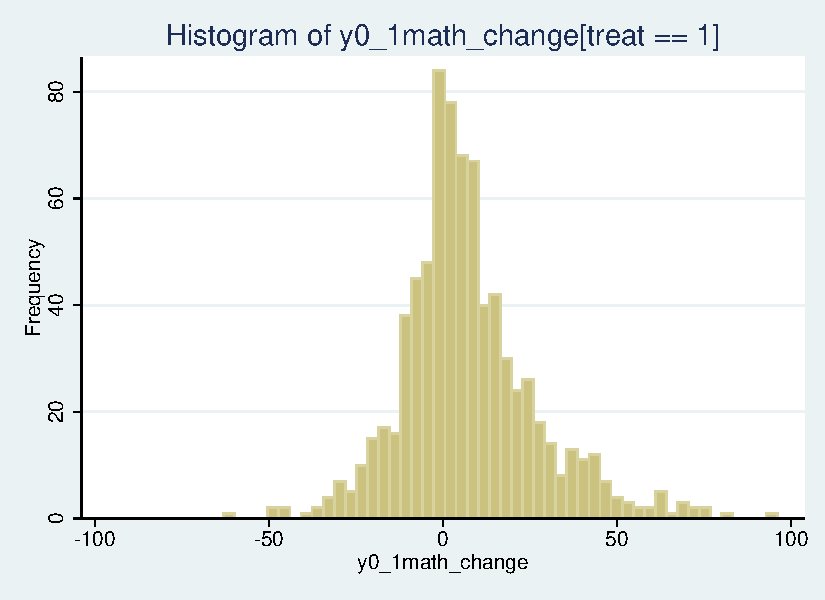
\includegraphics[width=5in,height=4in]{figure/PS12-unnamed-chunk-4-1} 

}

\end{knitrout}



\item To trim the top portion of the treatment group distribution, what value of $Y_i$ is the 93.6 percentile of the treatment group? (The value 93.6 is the control group reporting rate divided by the treatment group reporting rate.)\\
Answer:\\
\begin{knitrout}
\definecolor{shadecolor}{rgb}{0.969, 0.969, 0.969}\color{fgcolor}\begin{kframe}
    \begin{Verbatim}[commandchars=\\\{\}]
{\color{incolor}In [{\color{incolor}7}]:} \PY{k}{centile} y0\PYZus{}1math\PYZus{}change\PY{k}{ if} treat\PY{o}{==}\PY{l+m}{1},\PY{k}{ centile}(\PY{l+m}{93.6})
\end{Verbatim}

    \begin{Verbatim}[commandchars=\\\{\}]

                                                       -- Binom. Interp. --
    Variable |       Obs  Percentile    Centile        [95\% Conf. Interval]
-------------+-------------------------------------------------------------
y0\_1math\_c\textasciitilde{}e |       781       93.6          40              36          44

    \end{Verbatim}

\end{kframe}
\end{knitrout}

The 93.6 percentile value of Y is 40.

\item What is the average value of the treatment group observations that are less than the 93.6 percentile value? Call this average treatment effect $L_B$. Confirm that the percentage of the original treatment group that remains is equal to the percentage of the control group with outcome data.\\
Answer:\\
\begin{knitrout}
\definecolor{shadecolor}{rgb}{0.969, 0.969, 0.969}\color{fgcolor}\begin{kframe}
    \begin{Verbatim}[commandchars=\\\{\}]
{\color{incolor}In [{\color{incolor}8}]:} \PY{k}{qui}\PY{k}{ mean} y0\PYZus{}1math\PYZus{}change\PY{k}{ if} treat\PY{o}{==}\PY{l+m}{1} \PY{o}{\PYZam{}} missing\PYZus{}y1math\PY{o}{==}\PY{l+m}{0} \PY{o}{\PYZam{}} y0\PYZus{}1math\PYZus{}change \PY{o}{\PYZlt{}} \PY{l+m}{40}
        \PY{k}{scalar} l\PYZus{}b = \PYZus{}b[y0\PYZus{}1math\PYZus{}change]
        \PY{k}{qui}\PY{k}{ count}\PY{k}{ if} treat\PY{o}{==}\PY{l+m}{1} \PY{o}{\PYZam{}} missing\PYZus{}y1math\PY{o}{==}\PY{l+m}{0} \PY{o}{\PYZam{}} y0\PYZus{}1math\PYZus{}change \PY{o}{\PYZlt{}} \PY{l+m}{40}
        \PY{k}{scalar} l\PYZus{}b\PYZus{}count = \PY{n+nf}{r}(N)
        \PY{k}{qui}\PY{k}{ count}\PY{k}{ if} treat\PY{o}{==}\PY{l+m}{1}
\end{Verbatim}

    \begin{Verbatim}[commandchars=\\\{\}]
{\color{incolor}In [{\color{incolor}9}]:} \PY{k}{disp} \PY{n+nFormat}{\PYZpc{}8.6f} l\PYZus{}b
\end{Verbatim}

    \begin{Verbatim}[commandchars=\\\{\}]
3.701513

    \end{Verbatim}

    \begin{Verbatim}[commandchars=\\\{\}]
{\color{incolor}In [{\color{incolor}10}]:} \PY{k}{disp} \PY{n+nFormat}{\PYZpc{}8.7f} \PY{l+m}{1}\PY{o}{\PYZhy{}}l\PYZus{}b\PYZus{}count\PY{o}{/}\PY{n+nf}{r}(N)
\end{Verbatim}

    \begin{Verbatim}[commandchars=\\\{\}]
0.2450675

    \end{Verbatim}

\end{kframe}
\end{knitrout}

The average value of the observations less than or equal to 40 is 3.70. There are 727 such values, and  1- (727/963) = 24.5\%. The rate of missing for the control group is 24.1\%.  


\item Subtract the control group average from $L_B$.\\
Answer:\\
\begin{knitrout}
\definecolor{shadecolor}{rgb}{0.969, 0.969, 0.969}\color{fgcolor}\begin{kframe}
    \begin{Verbatim}[commandchars=\\\{\}]
{\color{incolor}In [{\color{incolor}11}]:} \PY{k}{qui}\PY{k}{ mean} y0\PYZus{}1math\PYZus{}change\PY{k}{ if} treat\PY{o}{==}\PY{l+m}{0} 
         \PY{k}{disp} \PY{n+nFormat}{\PYZpc{}18.6f} l\PYZus{}b \PY{o}{\PYZhy{}} \PYZus{}b[y0\PYZus{}1math\PYZus{}change]
\end{Verbatim}
    \begin{Verbatim}[commandchars=\\\{\}]
         -2.785134
    \end{Verbatim}
\end{kframe}
\end{knitrout}


\item To trim the bottom portion of the treatment group distribution, what treatment group outcome corresponds to the 6.4 percentile? (The value 6.4 is calculated by subtracting 93.6 from 100.)\\
Answer:\\
\begin{knitrout}
\definecolor{shadecolor}{rgb}{0.969, 0.969, 0.969}\color{fgcolor}\begin{kframe}
    \begin{Verbatim}[commandchars=\\\{\}]
{\color{incolor}In [{\color{incolor}12}]:} \PY{k}{centile} y0\PYZus{}1math\PYZus{}change\PY{k}{ if} treat\PY{o}{==}\PY{l+m}{1},\PY{k}{ centile}(\PY{l+m}{6.4})
\end{Verbatim}

    \begin{Verbatim}[commandchars=\\\{\}]

                                                       -- Binom. Interp. --
    Variable |       Obs  Percentile    Centile        [95\% Conf. Interval]
-------------+-------------------------------------------------------------
y0\_1math\_c\textasciitilde{}e |       781        6.4         -18             -21         -16

    \end{Verbatim}
\end{kframe}
\end{knitrout}
The 6.4 percentile value is -18. 

\item What is the average value of the treatment group observations that are greater than the 6.4 percentile? Call this average treatment $U_B$. Confirm that the percentage of the original treatment group that remains after trimming is equal to the percentage of the control group with outcome data.\\
Answer:\\

\begin{knitrout}
\definecolor{shadecolor}{rgb}{0.969, 0.969, 0.969}\color{fgcolor}\begin{kframe}
   \begin{Verbatim}[commandchars=\\\{\}]
{\color{incolor}In [{\color{incolor}13}]:} \PY{k}{qui}\PY{k}{ mean} y0\PYZus{}1math\PYZus{}change\PY{k}{ if} treat\PY{o}{==}\PY{l+m}{1} \PY{o}{\PYZam{}} missing\PYZus{}y1math\PY{o}{==}\PY{l+m}{0} \PY{o}{\PYZam{}} y0\PYZus{}1math\PYZus{}change \PY{o}{\PYZgt{}} \PY{o}{\PYZhy{}}\PY{l+m}{18}
         \PY{k}{scalar} u\PYZus{}b = \PYZus{}b[y0\PYZus{}1math\PYZus{}change]
         \PY{k}{disp} \PY{n+nFormat}{\PYZpc{}8.6f} u\PYZus{}b
\end{Verbatim}

    \begin{Verbatim}[commandchars=\\\{\}]
9.707586

    \end{Verbatim}

    \begin{Verbatim}[commandchars=\\\{\}]
{\color{incolor}In [{\color{incolor}14}]:} \PY{k}{qui}\PY{k}{ count}\PY{k}{ if} treat\PY{o}{==}\PY{l+m}{1} \PY{o}{\PYZam{}} missing\PYZus{}y1math\PY{o}{==}\PY{l+m}{0} \PY{o}{\PYZam{}} y0\PYZus{}1math\PYZus{}change \PY{o}{\PYZgt{}} \PY{o}{\PYZhy{}}\PY{l+m}{18}
         \PY{k}{scalar} u\PYZus{}b\PYZus{}count = \PY{n+nf}{r}(N)
         \PY{k}{qui}\PY{k}{ count}\PY{k}{ if} treat\PY{o}{==}\PY{l+m}{1}
         \PY{k}{disp} \PY{n+nFormat}{\PYZpc{}8.7f} \PY{l+m}{1}\PY{o}{\PYZhy{}}u\PYZus{}b\PYZus{}count\PY{o}{/}\PY{n+nf}{r}(N)
\end{Verbatim}

    \begin{Verbatim}[commandchars=\\\{\}]
0.2471443

    \end{Verbatim}
\end{kframe}
\end{knitrout}

The average of the values that remain after trimming off the lower 6.4\% is 9.71. The percentage of those reporting with outcomes greater than -18 is 725/963=75.3\% for a missing rate of 24.7\%. This is approximately equal to the missing rate for the control group of 24.1\%

\item Subtract the control group average from $U_B$.\\
Answer:\\
\begin{knitrout}
\definecolor{shadecolor}{rgb}{0.969, 0.969, 0.969}\color{fgcolor}\begin{kframe}
   \begin{Verbatim}[commandchars=\\\{\}]
{\color{incolor}In [{\color{incolor}15}]:} \PY{k}{qui}\PY{k}{ mean} y0\PYZus{}1math\PYZus{}change\PY{k}{ if} treat\PY{o}{==}\PY{l+m}{0} 
         \PY{k}{disp} \PY{n+nFormat}{\PYZpc{}8.6f} u\PYZus{}b \PY{o}{\PYZhy{}} \PYZus{}b[y0\PYZus{}1math\PYZus{}change]
\end{Verbatim}

    \begin{Verbatim}[commandchars=\\\{\}]
3.220939
    \end{Verbatim}
\end{kframe}
\end{knitrout}



\item The lower and upper bounds that you calculated in parts (f) and (i) are designed to bound an ATE for a particular subgroup. Describe this subgroup.\\
Answer:\\
(3.22, -2.79) are the estimated bounds for the treatment effect for the always reporters. 


\end{enumerate}

\section*{Question 12}
\begin{knitrout}
\definecolor{shadecolor}{rgb}{0.969, 0.969, 0.969}\color{fgcolor}\begin{kframe}
\begin{verbatim}






\end{verbatim}
\end{kframe}
\end{knitrout}


\end{document}

